% Created by tikzDevice version 0.10.1 on 2017-05-28 17:18:03
% !TEX encoding = UTF-8 Unicode
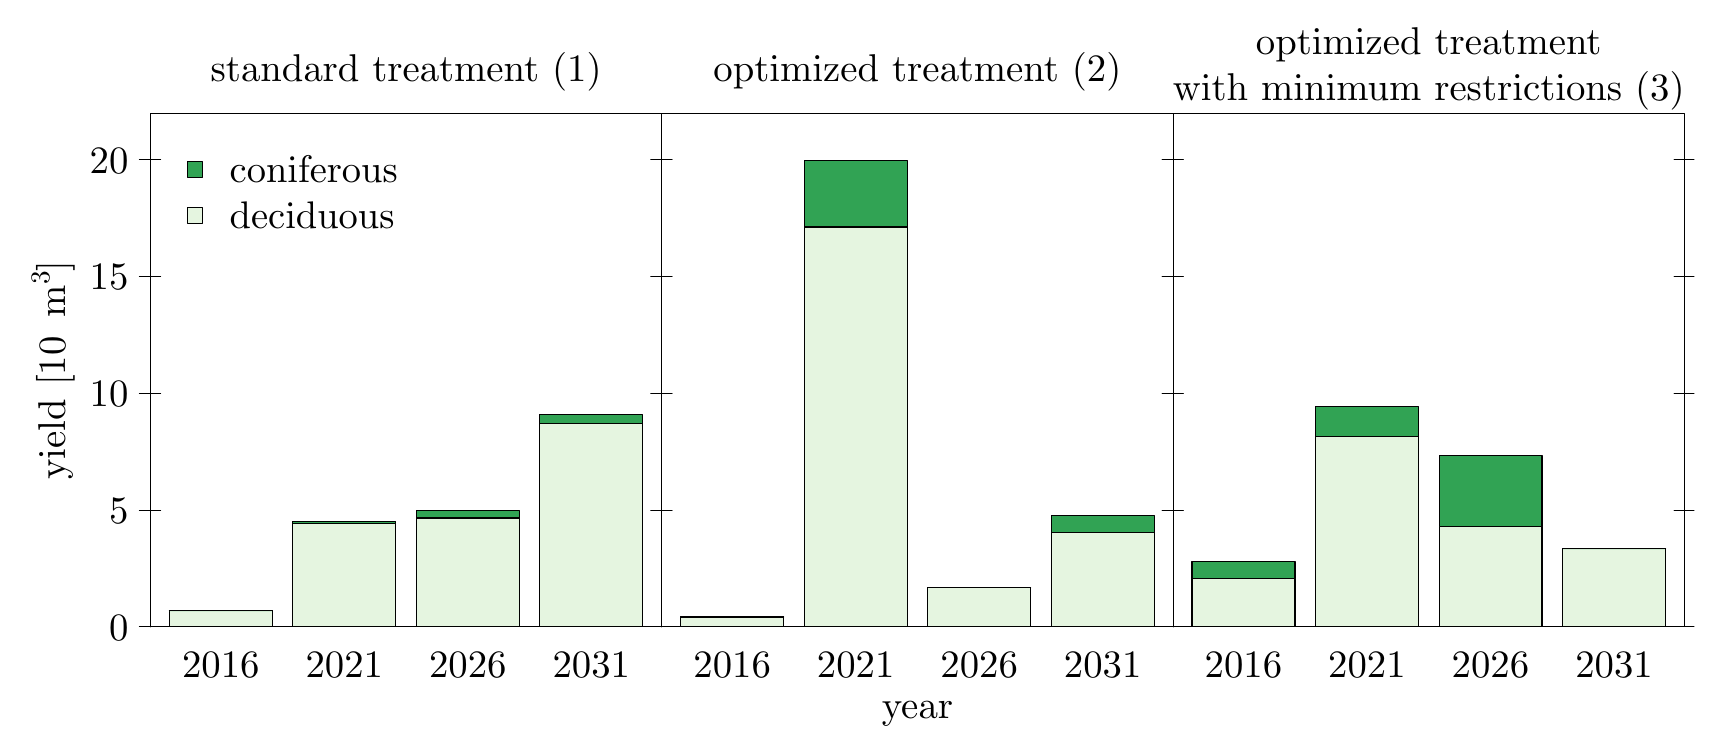
\begin{tikzpicture}[x=1pt,y=1pt]
\definecolor{fillColor}{RGB}{255,255,255}
\path[use as bounding box,fill=fillColor,fill opacity=0.00] (0,0) rectangle (602.23,252.94);
\begin{scope}
\path[clip] ( 44.35, 36.43) rectangle (229.12,222.06);
\definecolor{drawColor}{RGB}{0,0,0}
\definecolor{fillColor}{RGB}{229,245,224}

\path[draw=drawColor,line width= 0.4pt,line join=round,line cap=round,fill=fillColor] ( 51.20, 36.43) rectangle ( 88.39, 42.31);
\definecolor{fillColor}{RGB}{49,163,84}

\path[draw=drawColor,line width= 0.4pt,line join=round,line cap=round,fill=fillColor] ( 51.20, 42.31) rectangle ( 88.39, 42.31);
\definecolor{fillColor}{RGB}{229,245,224}

\path[draw=drawColor,line width= 0.4pt,line join=round,line cap=round,fill=fillColor] ( 95.83, 36.43) rectangle (133.02, 73.67);
\definecolor{fillColor}{RGB}{49,163,84}

\path[draw=drawColor,line width= 0.4pt,line join=round,line cap=round,fill=fillColor] ( 95.83, 73.67) rectangle (133.02, 74.64);
\definecolor{fillColor}{RGB}{229,245,224}

\path[draw=drawColor,line width= 0.4pt,line join=round,line cap=round,fill=fillColor] (140.46, 36.43) rectangle (177.65, 75.75);
\definecolor{fillColor}{RGB}{49,163,84}

\path[draw=drawColor,line width= 0.4pt,line join=round,line cap=round,fill=fillColor] (140.46, 75.75) rectangle (177.65, 78.43);
\definecolor{fillColor}{RGB}{229,245,224}

\path[draw=drawColor,line width= 0.4pt,line join=round,line cap=round,fill=fillColor] (185.09, 36.43) rectangle (222.28,109.94);
\definecolor{fillColor}{RGB}{49,163,84}

\path[draw=drawColor,line width= 0.4pt,line join=round,line cap=round,fill=fillColor] (185.09,109.94) rectangle (222.28,113.09);
\end{scope}
\begin{scope}
\path[clip] (  0.00,  0.00) rectangle (602.23,252.94);
\definecolor{drawColor}{RGB}{0,0,0}

\node[text=drawColor,anchor=base,inner sep=0pt, outer sep=0pt, scale=  1.40] at (136.74,233.66) {standard treatment (1)};

\path[draw=drawColor,line width= 0.4pt,line join=round,line cap=round] ( 44.35, 36.43) -- ( 40.39, 36.43);

\path[draw=drawColor,line width= 0.4pt,line join=round,line cap=round] ( 44.35, 78.62) -- ( 40.39, 78.62);

\path[draw=drawColor,line width= 0.4pt,line join=round,line cap=round] ( 44.35,120.81) -- ( 40.39,120.81);

\path[draw=drawColor,line width= 0.4pt,line join=round,line cap=round] ( 44.35,162.99) -- ( 40.39,162.99);

\path[draw=drawColor,line width= 0.4pt,line join=round,line cap=round] ( 44.35,205.18) -- ( 40.39,205.18);

\node[text=drawColor,anchor=base east,inner sep=0pt, outer sep=0pt, scale=  1.40] at ( 36.43, 31.61) {0};

\node[text=drawColor,anchor=base east,inner sep=0pt, outer sep=0pt, scale=  1.40] at ( 36.43, 73.80) {5};

\node[text=drawColor,anchor=base east,inner sep=0pt, outer sep=0pt, scale=  1.40] at ( 36.43,115.99) {10};

\node[text=drawColor,anchor=base east,inner sep=0pt, outer sep=0pt, scale=  1.40] at ( 36.43,158.17) {15};

\node[text=drawColor,anchor=base east,inner sep=0pt, outer sep=0pt, scale=  1.40] at ( 36.43,200.36) {20};

\path[draw=drawColor,line width= 0.4pt,line join=round,line cap=round] ( 44.35, 36.43) -- ( 48.05, 36.43);

\path[draw=drawColor,line width= 0.4pt,line join=round,line cap=round] ( 44.35, 78.62) -- ( 48.05, 78.62);

\path[draw=drawColor,line width= 0.4pt,line join=round,line cap=round] ( 44.35,120.81) -- ( 48.05,120.81);

\path[draw=drawColor,line width= 0.4pt,line join=round,line cap=round] ( 44.35,162.99) -- ( 48.05,162.99);

\path[draw=drawColor,line width= 0.4pt,line join=round,line cap=round] ( 44.35,205.18) -- ( 48.05,205.18);

\node[text=drawColor,anchor=base,inner sep=0pt, outer sep=0pt, scale=  1.40] at ( 69.79, 18.22) {2016};

\node[text=drawColor,anchor=base,inner sep=0pt, outer sep=0pt, scale=  1.40] at (114.42, 18.22) {2021};

\node[text=drawColor,anchor=base,inner sep=0pt, outer sep=0pt, scale=  1.40] at (159.05, 18.22) {2026};

\node[text=drawColor,anchor=base,inner sep=0pt, outer sep=0pt, scale=  1.40] at (203.68, 18.22) {2031};

\node[text=drawColor,rotate= 90.00,anchor=base west,inner sep=0pt, outer sep=0pt, scale=  1.40] at ( 13.53, 89.67) {yield [10};

\node[text=drawColor,rotate= 90.00,anchor=base west,inner sep=0pt, outer sep=0pt, scale=  1.40] at ( 13.53,141.37) { };

\node[text=drawColor,rotate= 90.00,anchor=base west,inner sep=0pt, outer sep=0pt, scale=  1.40] at ( 13.53,148.37) {m};

\node[text=drawColor,rotate= 90.00,anchor=base west,inner sep=0pt, outer sep=0pt, scale=  0.98] at (  7.80,160.04) {3};

\node[text=drawColor,rotate= 90.00,anchor=base west,inner sep=0pt, outer sep=0pt, scale=  1.40] at ( 13.53,164.94) {]};
\end{scope}
\begin{scope}
\path[clip] ( 44.35, 36.43) rectangle (229.12,222.06);
\definecolor{drawColor}{RGB}{0,0,0}
\definecolor{fillColor}{RGB}{49,163,84}

\path[draw=drawColor,line width= 0.4pt,line join=round,line cap=round,fill=fillColor] ( 57.76,198.95) rectangle ( 63.29,204.48);
\definecolor{fillColor}{RGB}{229,245,224}

\path[draw=drawColor,line width= 0.4pt,line join=round,line cap=round,fill=fillColor] ( 57.76,182.32) rectangle ( 63.29,187.84);

\node[text=drawColor,anchor=base west,inner sep=0pt, outer sep=0pt, scale=  1.39] at ( 73.00,196.94) {coniferous};

\node[text=drawColor,anchor=base west,inner sep=0pt, outer sep=0pt, scale=  1.39] at ( 73.00,180.31) {deciduous};
\end{scope}
\begin{scope}
\path[clip] (  0.00,  0.00) rectangle (602.23,252.94);
\definecolor{drawColor}{RGB}{0,0,0}

\path[draw=drawColor,line width= 0.4pt,line join=round,line cap=round] ( 44.35, 36.43) --
	(229.12, 36.43) --
	(229.12,222.06) --
	( 44.35,222.06) --
	( 44.35, 36.43);
\end{scope}
\begin{scope}
\path[clip] (229.12, 36.43) rectangle (413.89,222.06);
\definecolor{drawColor}{RGB}{0,0,0}
\definecolor{fillColor}{RGB}{229,245,224}

\path[draw=drawColor,line width= 0.4pt,line join=round,line cap=round,fill=fillColor] (235.97, 36.43) rectangle (273.16, 39.99);
\definecolor{fillColor}{RGB}{49,163,84}

\path[draw=drawColor,line width= 0.4pt,line join=round,line cap=round,fill=fillColor] (235.97, 39.99) rectangle (273.16, 39.99);
\definecolor{fillColor}{RGB}{229,245,224}

\path[draw=drawColor,line width= 0.4pt,line join=round,line cap=round,fill=fillColor] (280.60, 36.43) rectangle (317.79,180.91);
\definecolor{fillColor}{RGB}{49,163,84}

\path[draw=drawColor,line width= 0.4pt,line join=round,line cap=round,fill=fillColor] (280.60,180.91) rectangle (317.79,204.90);
\definecolor{fillColor}{RGB}{229,245,224}

\path[draw=drawColor,line width= 0.4pt,line join=round,line cap=round,fill=fillColor] (325.23, 36.43) rectangle (362.42, 50.69);
\definecolor{fillColor}{RGB}{49,163,84}

\path[draw=drawColor,line width= 0.4pt,line join=round,line cap=round,fill=fillColor] (325.23, 50.69) rectangle (362.42, 50.69);
\definecolor{fillColor}{RGB}{229,245,224}

\path[draw=drawColor,line width= 0.4pt,line join=round,line cap=round,fill=fillColor] (369.86, 36.43) rectangle (407.05, 70.62);
\definecolor{fillColor}{RGB}{49,163,84}

\path[draw=drawColor,line width= 0.4pt,line join=round,line cap=round,fill=fillColor] (369.86, 70.62) rectangle (407.05, 76.80);
\end{scope}
\begin{scope}
\path[clip] (  0.00,  0.00) rectangle (602.23,252.94);
\definecolor{drawColor}{RGB}{0,0,0}

\path[draw=drawColor,line width= 0.4pt,line join=round,line cap=round] (229.12, 36.43) -- (225.16, 36.43);

\path[draw=drawColor,line width= 0.4pt,line join=round,line cap=round] (229.12, 78.62) -- (225.16, 78.62);

\path[draw=drawColor,line width= 0.4pt,line join=round,line cap=round] (229.12,120.81) -- (225.16,120.81);

\path[draw=drawColor,line width= 0.4pt,line join=round,line cap=round] (229.12,162.99) -- (225.16,162.99);

\path[draw=drawColor,line width= 0.4pt,line join=round,line cap=round] (229.12,205.18) -- (225.16,205.18);

\path[draw=drawColor,line width= 0.4pt,line join=round,line cap=round] (229.12, 36.43) -- (232.82, 36.43);

\path[draw=drawColor,line width= 0.4pt,line join=round,line cap=round] (229.12, 78.62) -- (232.82, 78.62);

\path[draw=drawColor,line width= 0.4pt,line join=round,line cap=round] (229.12,120.81) -- (232.82,120.81);

\path[draw=drawColor,line width= 0.4pt,line join=round,line cap=round] (229.12,162.99) -- (232.82,162.99);

\path[draw=drawColor,line width= 0.4pt,line join=round,line cap=round] (229.12,205.18) -- (232.82,205.18);

\node[text=drawColor,anchor=base,inner sep=0pt, outer sep=0pt, scale=  1.40] at (254.56, 18.22) {2016};

\node[text=drawColor,anchor=base,inner sep=0pt, outer sep=0pt, scale=  1.40] at (299.19, 18.22) {2021};

\node[text=drawColor,anchor=base,inner sep=0pt, outer sep=0pt, scale=  1.40] at (343.82, 18.22) {2026};

\node[text=drawColor,anchor=base,inner sep=0pt, outer sep=0pt, scale=  1.40] at (388.45, 18.22) {2031};

\path[draw=drawColor,line width= 0.4pt,line join=round,line cap=round] (229.12, 36.43) --
	(413.89, 36.43) --
	(413.89,222.06) --
	(229.12,222.06) --
	(229.12, 36.43);

\node[text=drawColor,anchor=base,inner sep=0pt, outer sep=0pt, scale=  1.40] at (321.51,233.66) {optimized treatment (2)};

\node[text=drawColor,anchor=base,inner sep=0pt, outer sep=0pt, scale=  1.40] at (321.51,  3.17) {year};
\end{scope}
\begin{scope}
\path[clip] (413.89, 36.43) rectangle (598.66,222.06);
\definecolor{drawColor}{RGB}{0,0,0}
\definecolor{fillColor}{RGB}{229,245,224}

\path[draw=drawColor,line width= 0.4pt,line join=round,line cap=round,fill=fillColor] (420.74, 36.43) rectangle (457.93, 53.86);
\definecolor{fillColor}{RGB}{49,163,84}

\path[draw=drawColor,line width= 0.4pt,line join=round,line cap=round,fill=fillColor] (420.74, 53.86) rectangle (457.93, 59.96);
\definecolor{fillColor}{RGB}{229,245,224}

\path[draw=drawColor,line width= 0.4pt,line join=round,line cap=round,fill=fillColor] (465.37, 36.43) rectangle (502.56,105.28);
\definecolor{fillColor}{RGB}{49,163,84}

\path[draw=drawColor,line width= 0.4pt,line join=round,line cap=round,fill=fillColor] (465.37,105.28) rectangle (502.56,116.05);
\definecolor{fillColor}{RGB}{229,245,224}

\path[draw=drawColor,line width= 0.4pt,line join=round,line cap=round,fill=fillColor] (510.00, 36.43) rectangle (547.19, 72.60);
\definecolor{fillColor}{RGB}{49,163,84}

\path[draw=drawColor,line width= 0.4pt,line join=round,line cap=round,fill=fillColor] (510.00, 72.60) rectangle (547.19, 98.36);
\definecolor{fillColor}{RGB}{229,245,224}

\path[draw=drawColor,line width= 0.4pt,line join=round,line cap=round,fill=fillColor] (554.63, 36.43) rectangle (591.82, 64.58);
\definecolor{fillColor}{RGB}{49,163,84}

\path[draw=drawColor,line width= 0.4pt,line join=round,line cap=round,fill=fillColor] (554.63, 64.58) rectangle (591.82, 64.58);
\end{scope}
\begin{scope}
\path[clip] (  0.00,  0.00) rectangle (602.23,252.94);
\definecolor{drawColor}{RGB}{0,0,0}

\path[draw=drawColor,line width= 0.4pt,line join=round,line cap=round] (413.89, 36.43) -- (409.93, 36.43);

\path[draw=drawColor,line width= 0.4pt,line join=round,line cap=round] (413.89, 78.62) -- (409.93, 78.62);

\path[draw=drawColor,line width= 0.4pt,line join=round,line cap=round] (413.89,120.81) -- (409.93,120.81);

\path[draw=drawColor,line width= 0.4pt,line join=round,line cap=round] (413.89,162.99) -- (409.93,162.99);

\path[draw=drawColor,line width= 0.4pt,line join=round,line cap=round] (413.89,205.18) -- (409.93,205.18);

\path[draw=drawColor,line width= 0.4pt,line join=round,line cap=round] (413.89, 36.43) -- (417.59, 36.43);

\path[draw=drawColor,line width= 0.4pt,line join=round,line cap=round] (413.89, 78.62) -- (417.59, 78.62);

\path[draw=drawColor,line width= 0.4pt,line join=round,line cap=round] (413.89,120.81) -- (417.59,120.81);

\path[draw=drawColor,line width= 0.4pt,line join=round,line cap=round] (413.89,162.99) -- (417.59,162.99);

\path[draw=drawColor,line width= 0.4pt,line join=round,line cap=round] (413.89,205.18) -- (417.59,205.18);

\path[draw=drawColor,line width= 0.4pt,line join=round,line cap=round] (598.66, 36.43) -- (602.23, 36.43);

\path[draw=drawColor,line width= 0.4pt,line join=round,line cap=round] (598.66, 78.62) -- (602.23, 78.62);

\path[draw=drawColor,line width= 0.4pt,line join=round,line cap=round] (598.66,120.81) -- (602.23,120.81);

\path[draw=drawColor,line width= 0.4pt,line join=round,line cap=round] (598.66,162.99) -- (602.23,162.99);

\path[draw=drawColor,line width= 0.4pt,line join=round,line cap=round] (598.66,205.18) -- (602.23,205.18);

\path[draw=drawColor,line width= 0.4pt,line join=round,line cap=round] (598.66, 36.43) -- (594.97, 36.43);

\path[draw=drawColor,line width= 0.4pt,line join=round,line cap=round] (598.66, 78.62) -- (594.97, 78.62);

\path[draw=drawColor,line width= 0.4pt,line join=round,line cap=round] (598.66,120.81) -- (594.97,120.81);

\path[draw=drawColor,line width= 0.4pt,line join=round,line cap=round] (598.66,162.99) -- (594.97,162.99);

\path[draw=drawColor,line width= 0.4pt,line join=round,line cap=round] (598.66,205.18) -- (594.97,205.18);

\node[text=drawColor,anchor=base,inner sep=0pt, outer sep=0pt, scale=  1.40] at (439.33, 18.22) {2016};

\node[text=drawColor,anchor=base,inner sep=0pt, outer sep=0pt, scale=  1.40] at (483.96, 18.22) {2021};

\node[text=drawColor,anchor=base,inner sep=0pt, outer sep=0pt, scale=  1.40] at (528.59, 18.22) {2026};

\node[text=drawColor,anchor=base,inner sep=0pt, outer sep=0pt, scale=  1.40] at (573.22, 18.22) {2031};

\node[text=drawColor,anchor=base,inner sep=0pt, outer sep=0pt, scale=  1.40] at (506.28,243.30) {optimized treatment};

\node[text=drawColor,anchor=base,inner sep=0pt, outer sep=0pt, scale=  1.40] at (506.28,226.50) {with minimum restrictions (3)};

\path[draw=drawColor,line width= 0.4pt,line join=round,line cap=round] (413.89, 36.43) --
	(598.66, 36.43) --
	(598.66,222.06) --
	(413.89,222.06) --
	(413.89, 36.43);
\end{scope}
\end{tikzpicture}
